%%% Title:    Categorical Code Interpretations
%%% Author:   Kyle M. Lang
%%% Created:  2021-03-23
%%% Modified: 2021-03-24

\documentclass{article}\usepackage[]{graphicx}\usepackage[]{color}
% maxwidth is the original width if it is less than linewidth
% otherwise use linewidth (to make sure the graphics do not exceed the margin)
\makeatletter
\def\maxwidth{ %
  \ifdim\Gin@nat@width>\linewidth
    \linewidth
  \else
    \Gin@nat@width
  \fi
}
\makeatother

\definecolor{fgcolor}{rgb}{0, 0, 0}
\newcommand{\hlnum}[1]{\textcolor[rgb]{0.69,0.494,0}{#1}}%
\newcommand{\hlstr}[1]{\textcolor[rgb]{0.749,0.012,0.012}{#1}}%
\newcommand{\hlcom}[1]{\textcolor[rgb]{0.514,0.506,0.514}{\textit{#1}}}%
\newcommand{\hlopt}[1]{\textcolor[rgb]{0,0,0}{#1}}%
\newcommand{\hlstd}[1]{\textcolor[rgb]{0,0,0}{#1}}%
\newcommand{\hlkwa}[1]{\textcolor[rgb]{0,0,0}{\textbf{#1}}}%
\newcommand{\hlkwb}[1]{\textcolor[rgb]{0,0.341,0.682}{#1}}%
\newcommand{\hlkwc}[1]{\textcolor[rgb]{0,0,0}{\textbf{#1}}}%
\newcommand{\hlkwd}[1]{\textcolor[rgb]{0.004,0.004,0.506}{#1}}%
\let\hlipl\hlkwb

\usepackage{framed}
\makeatletter
\newenvironment{kframe}{%
 \def\at@end@of@kframe{}%
 \ifinner\ifhmode%
  \def\at@end@of@kframe{\end{minipage}}%
  \begin{minipage}{\columnwidth}%
 \fi\fi%
 \def\FrameCommand##1{\hskip\@totalleftmargin \hskip-\fboxsep
 \colorbox{shadecolor}{##1}\hskip-\fboxsep
     % There is no \\@totalrightmargin, so:
     \hskip-\linewidth \hskip-\@totalleftmargin \hskip\columnwidth}%
 \MakeFramed {\advance\hsize-\width
   \@totalleftmargin\z@ \linewidth\hsize
   \@setminipage}}%
 {\par\unskip\endMakeFramed%
 \at@end@of@kframe}
\makeatother

\definecolor{shadecolor}{rgb}{.97, .97, .97}
\definecolor{messagecolor}{rgb}{0, 0, 0}
\definecolor{warningcolor}{rgb}{1, 0, 1}
\definecolor{errorcolor}{rgb}{1, 0, 0}
\newenvironment{knitrout}{}{} % an empty environment to be redefined in TeX

\usepackage{alltt}

\usepackage{graphicx}
\usepackage{booktabs}
\usepackage[natbibapa]{apacite}
\usepackage[libertine]{newtxmath}
\usepackage{fancybox}
\usepackage{datetime2}

\title{Interpreting the Intercept in Linear Regression Models with Categorical Predictors}
\author{Kyle M. Lang}
\IfFileExists{upquote.sty}{\usepackage{upquote}}{}
\begin{document}



\maketitle

In this document, I'll go through the interpretation of the estimated intercept
in multiple linear regression models that contain categorical predictors. The
interpretation of the intercept differs based on the nature of the variables on
the right hand side (RHS) of the regression equation. For simple linear
regression models, the following represent the intercept interpretations for
some common types of predictor variables.

\begin{itemize}
\item Continuous $X$: The model-implied mean of $Y$ (i.e., the expected value
  for $Y$, given our model) for cases with $X = 0$.
\item Dummy-coded $X$: The model-implied mean of $Y$ for cases in the reference
  group of $X$.
\item Unweighted effects-coded $X$: The model-implied, unweighted mean of $Y$
  (see below for definition of the unweighted mean)
\item Weighted effects-coded $X$: The model-implied, weighted mean of $Y$
  (see below for definition of the weighted mean)
\end{itemize}

When we combine different types of variables and/or codes on the RHS of a
multiple linear regression model, the intercept is interpreted as a sort of
``intersection'' of the interpretations for the separate variable types/codes.

\begin{itemize}
\item Dummy-coded $X_1$ and continuous $X_2$: The model-implied mean of $Y$ for
  cases in the reference group of $X_1$ with $X_2 = 0$.
\item Unweighted effects-coded $X_1$ and continuous $X_2$: The model-implied,
  unweighted mean of $Y$ for cases with $X_2 = 0$.
\item Weighted effects-coded $X_1$ and continuous $X_2$: The model-implied,
  weighted mean of $Y$ for cases with $X_2 = 0$.
\item Dummy-coded $X_1$ and unweighted effects-coded $X_2$: The model-implied,
  unweighted mean of $Y$ for cases in the reference group of $X_1$.
\item Dummy-coded $X_1$ and weighted effects-coded $X_2$: The model-implied,
  weighted mean of $Y$ for cases in the reference group of $X_1$.
\item Weighted effects-coded $X_1$ and unweighted effects-coded $X_2$: The
  model-implied mean of $Y$ calculated with proportional weighting across the
  groups of the $X_1$ factor and without weighting for the groups of the $X_2$
  factor.
\end{itemize}

Note that the final combination (e.g., both weighted and unweighted effects
codes) should not come up much, in practice. Usually, your data characteristics
or your inferential goals will motivate the use of either all weighted effects
codes or all unweighted effects codes. In the following section, I'll show a few
examples of the combined interpretations described above.

\section{Example Interpretations}

We'll anchor our interpretations by refitting the same model with different
coding schemes for the predictor variables. In our example model, we'll regress
BMI onto a two-level factor representing biological sex and a three-level factor
representing educational attainment level.
\begin{align*}
  Y_{\textit{bmi}} = 
  \beta_0 + 
  \beta_1X_{\textit{female}} + 
  \beta_2X_{\textit{ed.mid}} + 
  \beta_2X_{\textit{ed.hi}} + 
  \varepsilon
\end{align*}

We will use the \emph{BMI} data from the \textbf{wec} package \citep{wec} to fit
this model using different flavors of categorical coding for the \emph{sex} and
\emph{education} factors.

\subsection{Two Dummy Codes}



When coding each factor using dummy codes, we get the following fitted
regression equation.
\begin{align*}
  \hat{Y}_{\textit{bmi}} = 
  26.4 
  -0.5X_{\textit{female}} 
  -1.14X_{\textit{ed.mid}} 
  -1.86X_{\textit{ed.hi}}
\end{align*}
The male group is the reference group for the \emph{sex} factor, and the lowest
educational attainment group is the reference group for the \emph{education}
factor. So, the intercept, $\hat{\beta}_0 = 26.4$,
represents the model-implied mean of BMI (i.e., the expected BMI given our
fitted model) for males in the lowest educational attainment group.

\subsection{Two Unweighted Effects Codes}



When coding each factor using unweighted effects codes, we get the following
fitted regression equation.
\begin{align*}
  \hat{Y}_{\textit{bmi}} = 
  25.15 +
  0.25X_{\textit{female}} + 
  1X_{\textit{ed.mid}} 
  -0.14X_{\textit{ed.hi}}
\end{align*}
In this case, we don't need to worry about keeping track of the reference groups
because the intercept represents the (unweighted) grand mean of BMI. Since both
factors are coded with unweighted effects codes, the model-implied, unweighted
mean of BMI is $\hat{\beta}_0 = 25.15$.

\subsubsection{What is the Unweighted Mean?}
For this model, the unweighted mean is defined as the simple average of the
group-specific means of BMI. Since the \emph{sex} factor has two levels and the
\emph{education} factor has three levels, we have $2 \times 3 = 6$
group-specific means.

% latex table generated in R 4.0.4 by xtable 1.8-4 package
% Wed Mar 24 22:03:07 2021
\begin{table}[ht]
\centering
\begin{tabular}{rrrr}
  \toprule
 & highest & middle & lowest \\ 
  \midrule
female & 26.07 & 25.29 & 24.71 \\ 
  male & 26.22 & 24.74 & 23.89 \\ 
   \bottomrule
\end{tabular}
\caption{Group-Specific Means of BMI} 
\label{mTab}
\end{table}


Averaging these six group-specific means produces the unweighted mean of BMI
($\overline{\textit{BMI}} = 25.15$). We call this
quantity the \emph{unweighted} mean because we compute it as the simple average
of the group-specific means (i.e., we don't weight the means by their relative
sample sizes).

\subsection{Two Weighted Effects Codes}



When coding each factor using weighted effects codes, we get the following
fitted regression equation.
\begin{align*}
  \hat{Y}_{\textit{bmi}} = 
  24.98 
  -0.23X_{\textit{female}} + 
  0.02X_{\textit{ed.mid}} 
  -0.7X_{\textit{ed.hi}}
\end{align*}
Again, we don't need to concern ourselves with the reference groups because the
intercept represents the (weighted) grand mean of BMI. Since both factors are
coded with weighted effects codes, the model-implied, weighted mean of BMI is
$\hat{\beta}_0 = 24.98$.

\subsubsection{What is the Weighted Mean?}
In this case, the weighted mean is defined as the weighted average of the
group-specific means of BMI. We weight the group-specific means shown in Table
\ref{mTab} by weights representing the proportion of the total sample size
associated with each group.

% latex table generated in R 4.0.4 by xtable 1.8-4 package
% Wed Mar 24 22:03:07 2021
\begin{table}[ht]
\centering
\begin{tabular}{rrrr}
  \toprule
 & lowest & middle & highest \\ 
  \midrule
male & 0.103 & 0.187 & 0.181 \\ 
  female & 0.107 & 0.241 & 0.180 \\ 
   \bottomrule
\end{tabular}
\caption{Group-Specific Sample Weights} 
\label{wTab}
\end{table}


To compute the weighted mean, assume we have two matrices such as those shown in
Tables \ref{mTab} and \ref{wTab}:
\begin{itemize}
\item An $L \times K$ matrix of group-specific means of $Y$, $M$, with elements
  $m_{lk}$
\item The corresponding matrix of group-specific sample weights, $W$, with
  elements $w_{lk}$
\end{itemize}
We can then compute the weighted mean of $Y$ via the following formula:
\begin{align*}
  \bar{Y} = \sum_{l = 1}^L \sum_{k = 1}^K w_{lk} m_{lk}
\end{align*}
For our example data, the estimated weighted mean is $\overline{\textit{BMI}} =
24.98$. When computing this quantity from the raw
data, the weighted mean of $Y$ will equal the arithmetic average of $Y$,
$\bar{Y} = N^{-1} \sum_{n = 1}^N y_n$.

\subsection{Dummy Code and Unweighted Effects Code}



When we code \emph{sex} with a dummy code and \emph{education} with unweighted
effects codes, we get the following fitted regression equation.
\begin{align*}
  \hat{Y}_{\textit{bmi}} = 
  25.4
  -0.5X_{\textit{female}} + 
  1X_{\textit{ed.mid}} 
  -0.14X_{\textit{ed.hi}}
\end{align*}
The reference groups for \emph{sex} is still males. So, the intercept,
$\hat{\beta}_0 = 25.4$, represents the model-implied,
unweighted mean of BMI for males. To compute the analogous marginal mean from
the raw data, we would simply average the three group-specific means in the
first row of Table \ref{mTab}.

\subsection{Dummy Code and Weighted Effects Code}



When coding \emph{sex} with a dummy code and \emph{education} with weighted
effects codes, we get the following fitted regression equation.
\begin{align*}
  \hat{Y}_{\textit{bmi}} = 
  25.24 
  -0.5X_{\textit{female}} + 
  0.02X_{\textit{ed.mid}} 
  -0.7X_{\textit{ed.hi}}
\end{align*}
Here, the intercept, $\hat{\beta}_0 = 25.24$, represents the
model-implied, weighted mean of BMI for males. To compute the analogous marginal
mean from the raw data, we would weight the three group-specific means in the
first row of Table \ref{mTab} by the corresponding sample weights in the first
row of Table \ref{wTab} and sum these products.

\section{Estimated Intercepts $\neq$ Data-Derived Means?}

Often, the estimated intercept from a given model does not match the
corresponding marginal mean that we would calculate from the raw data. We can
see an example of this discordance if we review the example with two dummy-coded
predictors from above. When we use dummy codes for both the \emph{sex} and
\emph{education} factors, we get an estimated intercept of $\hat{\beta}_0 =
26.402$, but the corresponding marginal mean from Table
\ref{mTab} is $\overline{\textit{BMI}}_{male,ed.low} = 26.074 \neq \hat{\beta}_0$.

Although this discordance may be disturbing, we don't really need to worry about
it. Remember that, for this example, the intercept is the \emph{model-implied}
mean of males in the lowest educational group. Our model does not perfectly
reproduce our data, though, so there can be discrepancies. If we estimate the
appropriate marginal means using our fitted model \citep[e.g., by using the
  \textbf{emmeans} package,][]{emmeans}, we see that the relevant marginal mean
estimated from our fitted model matches the estimated intercept.

% latex table generated in R 4.0.4 by xtable 1.8-4 package
% Wed Mar 24 22:03:08 2021
\begin{table}[ht]
\centering
\begin{tabular}{rrrr}
  \toprule
 & lowest & middle & highest \\ 
  \midrule
male & 26.40 & 25.26 & 24.55 \\ 
  female & 25.90 & 24.76 & 24.05 \\ 
   \bottomrule
\end{tabular}
\caption{Marginal Means Estimated from the Model} 
\label{mmTab}
\end{table}




\subsection{How is this Possible?}

To get some intuition for how the discordance between the model-based estimates
and the data-derived quantities can occur, consider the following figure.

\vspace{12pt}

\begin{knitrout}\footnotesize
\definecolor{shadecolor}{rgb}{0.878, 0.918, 0.933}\color{fgcolor}

{\centering 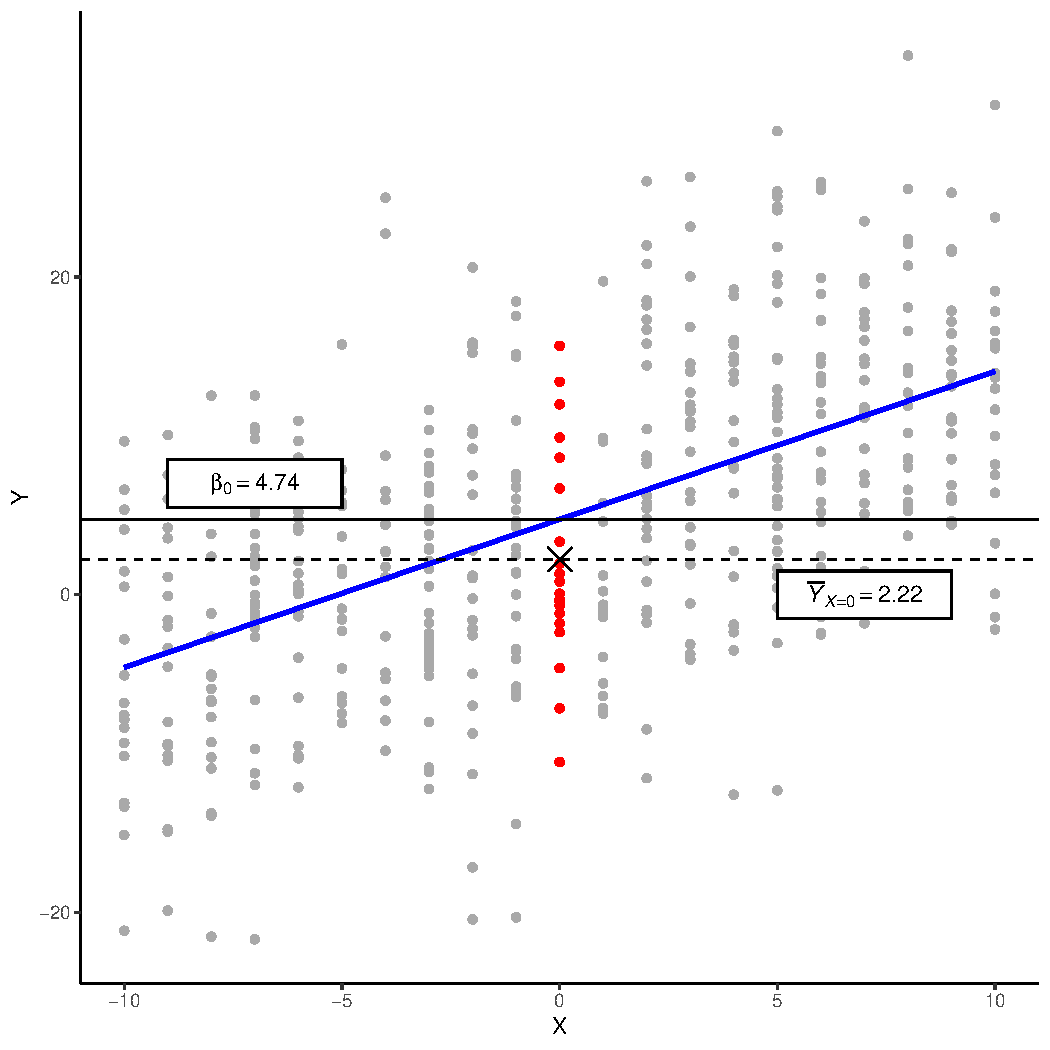
\includegraphics[width=0.85\linewidth]{figure/unnamed-chunk-10-1} 

}



\end{knitrout}

The above figure shows a scatterplot of $Y$ against $X$ with the fitted
regression line overlaid. Notice that the estimated intercept is $\hat{\beta}_0
= 4.74$. If, however, we average all of the $Y$ values for
which $X = 0$ (i.e., the red points in the figure), we get an estimated mean of
$Y_{X = 0} = 2.22 \neq \hat{\beta}_0$. Although these two
quantities share the same interpretation, they need not match in
practice. Regardless of what types of predictors are included, the model from
which the intercept is derived is only approximating the ideal relationship
between $X$ and $Y$. So, the estimated intercept may not match the analogous
quantity estimated directly from the raw data.

\bibliographystyle{apacite}
\bibliography{references.bib}


\end{document}
